% !Mode:: "TeX::UTF-8"

\documentclass{svk_short_sk}
\usepackage{graphicx}
\usepackage{caption}
\usepackage{subcaption}
\usepackage{float}

%% ak pisete po anglicky, pouzijete namiesto horneho riadku
%% \documentclass{svk_short_en}

\begin{document}
\title{Zarovnávanie sekvencií s~použitím metód klasifikácie}

\author{Michal Hozza
\email{Michal.Hozza@ksp.sk}
}
%% vsimnite si, ze u autorov sa nepisu tituly
%% prikaz \inst sluzi ako odkaz do zoznamu institucii
%% (vid. nizsie)

%% skolitela nepiste medzi autorov, ale v tejto casti
%% ak praca nema skolitela, jednoducho vynechajte
\supervisor{Tomáš Vinař\inst{1}
\email{vinar@fmph.uniba.sk}
, Michal N\'an\'asi\inst{2}
\email{mic@compbio.fmph.uniba.sk}
}

%% nasleduje kratka verzia nazvu clanku a
%% zoznam autorov (bez krstnych mien)
%% tieto informacie sa zobrazuju v hlavicke
\titlerunning{Zarovnávanie sekvencií s~použitím metód klasifikácie}
\authorrunning{Hozza}

\institute{
Katedra aplikovanej informatiky,
FMFI UK,
Mlynská Dolina
842~48~Bratislava
\and
Katedra informatiky,
FMFI UK,
Mlynská Dolina
842~48~Bratislava}

\maketitle

Zarovnávanie dvoch DNA sekvencií je jedným zo základných
bioinformatických problémov. Správne zarovnanie identifikuje časti
sekvencie, ktoré vznikli z~toho istého predka (zarovnané bázy), ako aj
inzercie a delécie v~priebehu evolúcie (medzery v~zarovnaní). Obvykle
takéto zarovnanie hľadáme pomocou jednoduchých párových skrytých
Markovovských modelov (pHMM) \cite{durbin}. V~tejto práci sa zaoberáme
možnosťami použitia prídavnej informácie o~funkcii vstupných sekvencií
(tzv. anotácie) na zlepšenie kvality takýchto zarovnaní.

\paragraph{Klasifikácia na základe lokálnej informácie.}

Informácie sme zakomponovali pomocou klasifikátorov, ktoré rozhodujú či dané pozície majú byť zarovnané k~sebe alebo nie. Ako klasifikátor sme použili \emph{RandomForest} \cite{randomForestPaper}, pretože aktuálne patrí medzi najlepšie klasifikátory.

Vstupné dáta pre klasifikátor sú okná veľkosti $w$, v ktorom sa nachádza $w$ dvojíc báz v okolí daných pozícií a ich anotácie (napr. či ide o gén alebo nie). Výstup je hodnota z intervalu $\left<0,1\right>$, ktorá označuje istotu klasifikátora, že dané dve pozície majú byť zarovnané k sebe (v insert stave, že daná pozícia má byť zarovnaná k medzere).

Ukázalo sa, že klasifikátor sa dokáže naučiť, ktoré okná majú byť zarovnané k~sebe a ktoré nie (Obr. \ref{fig:clf-m-dist}).

\begin{figure}[H]
    \centering
    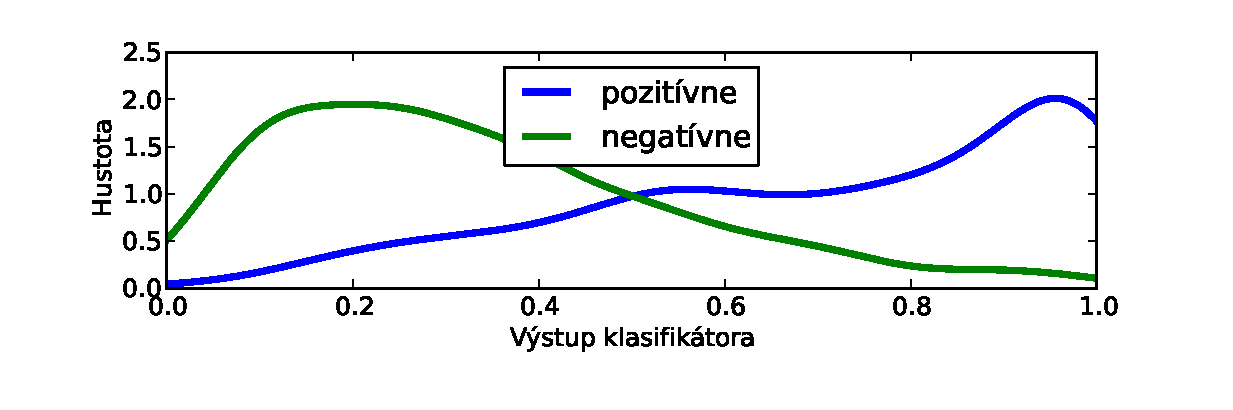
\includegraphics[width=.5\textwidth, clip=true]{images/clf_m_test}
    \caption{Distribúcia výstupu klasifikátora pre pozitívne a negatívne príklady. Pozitívne príklady sú tie, ktoré majú byť zarovnané k~sebe, negatívne príklady sú tie, ktoré k sebe zarovnané byť nemajú.}
    \label{fig:clf-m-dist}
\end{figure}

\paragraph{Zakomponovanie výsledkov klasifikácie do pHMM.}

Vyvinuli sme 2 modely pre zarovnanie sekvencií s~anotáciami za pomoci klasifikátora, ktoré sú založené na párových skrytých Markovovských modeloch.

\textbf{Model s~klasifikátorom ako emisiou:} (Obr. \ref{fig:model-clf})
V~tomto modeli sme nahradili emisné tabuľky stavov výstupom z~klasifikátora.
Model však nie je korektný pravdepodobnostný model, pretože pravdepodobnosti emisií nesčitujú do~1.

Emisné pravdepodobnosti sme prevzali priamo z klasifikátora, ktorý trénujeme zvlášť. Prechodové pravdepodobnosti sme natrénovali zo zarovnaní z trénovacej vzorky.

\textbf{Model s~klasifikátorovou páskou:} (Obr. \ref{fig:model-clf-tape})
Aby sme vyriešili problém s~korektnosťou predošlého modelu, navrhli sme alternatívu, ktorá navyše modeluje aj výstup z~klasifikátora.
Nemodelujeme teda len dvojicu sekvencií, ale aj sekvenciu výstupov klasifikátora.

V tomto modeli sme trénovali všetky parametre na trénovacej vzorke zarovnaní obohatenej o pásku s výstupmi z klasifikátora.

\begin{figure}[H]
        \centering
        \begin{subfigure}[b]{0.17\textwidth}
                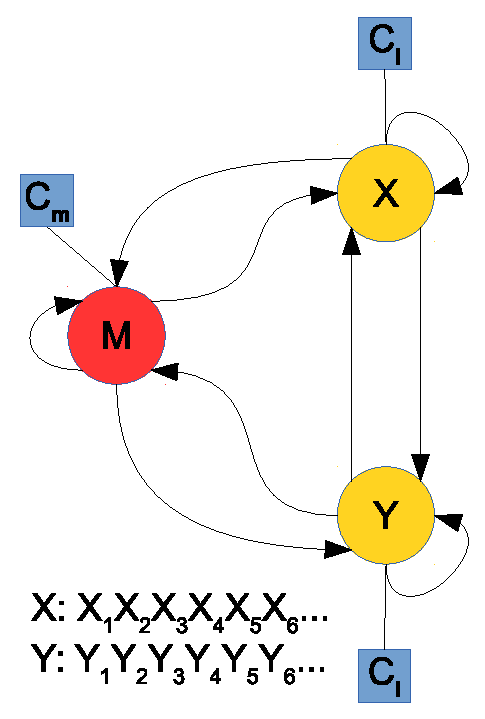
\includegraphics[width=\textwidth, clip=true]{images/model_clf}
                % \caption{Model s~klasifikátorom ako emisiou}
                \caption{}
                \label{fig:model-clf}
        \end{subfigure}%
        \qquad %add desired spacing between images, e. g. ~, \quad, \qquad etc.
          %(or a blank line to force the subfigure onto a new line)
        \begin{subfigure}[b]{0.17\textwidth}
                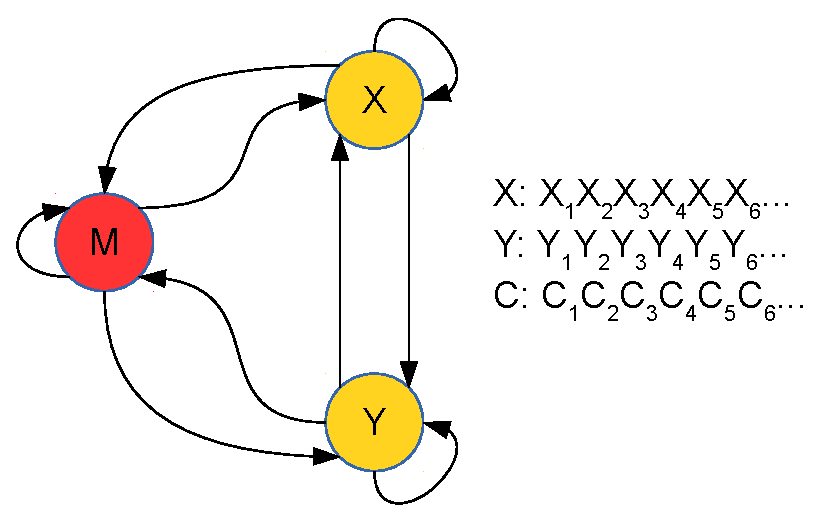
\includegraphics[width=\textwidth, clip=true]{images/model_clf_paska}
                % \caption{Model s~klasifikátorovou páskou}
                \caption{}
                \label{fig:model-clf-tape}
        \end{subfigure}
        \caption{Modely s~klasifikátorom}
\end{figure}
\vspace{-1cm}
% \nocite{*}
\bibliographystyle{apalike}
\bibliography{references}

%% citacie ulozte do suboru references.bib
%% na populaciu zoznamu literatury pouzite program
%%
%% bibtex references
%%
%% po ktorom je potrebne dokument znova zlatexovat

\end{document}
